

%---------------------------------------------
%
%       START
%
%---------------------------------------------

\chapter[Spatio-temporal disparity in mammals at the K-Pg boundary]{Spatio-temporal disparity in mammals at the K-Pg boundary}
\label{chap:STD_paper}

\bigskip
\begin{center}

\noindent{\Large \bf Mammalian morphological diversity does not increase in response to the Cretaceous-Paleogene event and the extinction of the (non-avian) dinosaurs.}
\footnote{A similar version of this chapter has been submitted to PLoS Biology (30/09/2015).}\footnote{\textit{Author contributions}: I designed the study, collected the data, ran the analyses and wrote the paper. NC helped design the study and commented on drafts of the manuscript.} \\

\begin{figure}[h]
  \centering
  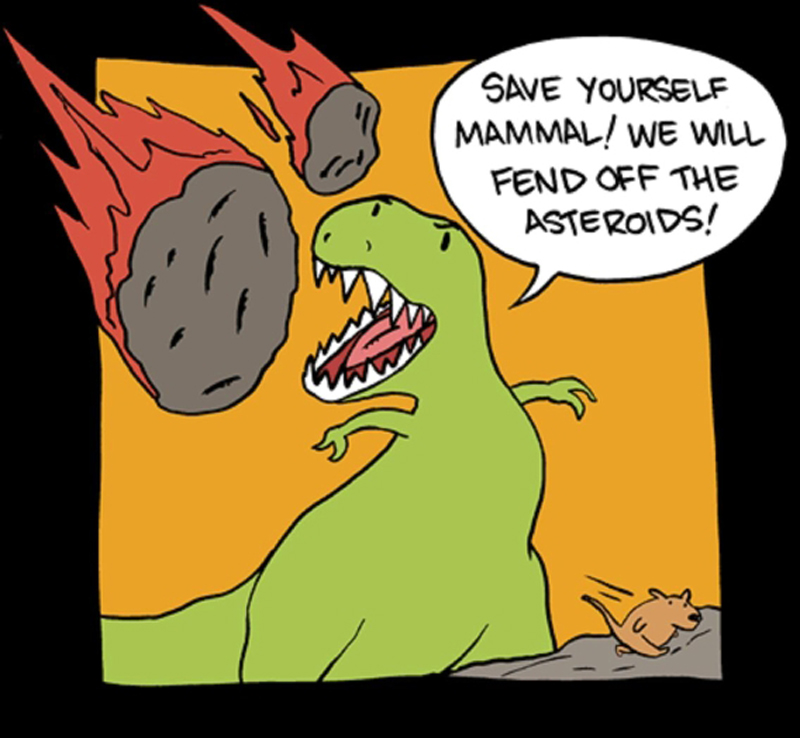
\includegraphics[width=0.8\textwidth]{STD/Figures/SMBC-ZachWeinersmith.jpg}
  \caption*{smbc-comics.com/?id=1535 -- \copyright SMBC Zach Weinersmith}
\end{figure}

\begin{quoteshrink}
  ``The most erroneous stories are those we think we know best - and therefore never scrutinize or question.''
\hfill{S.J. Gould}
\end{quoteshrink}
\bigskip

%} \\
% \medskip
% \noindent Key words: Total Evidence method, data structure, phylogenetic, fossil, topology\\
% \bigskip
% \noindent A shorter version (2500 words) will be submitted to Biology Letters as an invited submission for a special issue on phylogenies with living and fossil species. This special issue is open to submission in December 2015.\\

\end{center}
%---------------------------------------------
%
%       ABSTRACT
%
%---------------------------------------------
